\documentclass{article}
\usepackage[utf8]{inputenc}
\usepackage{longtable}
\usepackage{pgfplots}
\usepackage{amsfonts}
\usepackage{graphicx}
\usepackage{fullpage}
\usepackage{multicol}
\usepackage{amsmath}
\usepackage{amssymb}
\usepackage{natbib}

\pgfplotsset{compat=newest}
\title{Linear Regression}
\author{TDung}
\date{------------------------------------------}

\begin{document}
\tableofcontents

\maketitle
\section{Introduction}
  
	Linear regression is used to predict value of a variable based on the value of another one. The variable used to predict the other one is called \textit{Independent variable} (or sometimes, it might be called \textit{predictor variable}). The predicted variable is called \textit{dependent variable} (or sometimes, it might be called \textit{the outcome variable}).
	
    For example, you can use linear regression to predict the population of a country based on the population of previous years or maybe you can predict a person's height depends on their weight...
    
    In case we have more than one independent variable, we have to use multiple regression.
    
\section{The model behind linear regression} 
	\textit{Simple linear regression} model includes the \textit{mean function}(1) and the \textit{variance function}(2). 
	\begin{align}
            &E = (Y|X=x) = \beta _{0} + \beta _{1} x \\
            &Var(Y|X=x) = \sigma ^ {2}
    \end{align}
    In this line, Y is the output variable we want to predict, X is the input variable we know, $\beta_{0}$ and $\beta_{1}$ are the coefficients we need to estimate that can move the line around.
    
    The parameters in the \textit{mean function} (1) are the intercept ${\beta _{0}}$ and the slope ${\beta_{1}}$. The intercept is the value of ${E(Y |X = x)}$ when x equals to zero (\textit{in machine learning, it is called the bias, because it is added to offset all predictions}) and the slope is defined by the change in ${E(Y |X = x)}$ for a unit change in X. The parameters are usually unknown and must be estimated by using data. By changing the parameters, we can get all possible straight lines.
    
    \begin{center}
        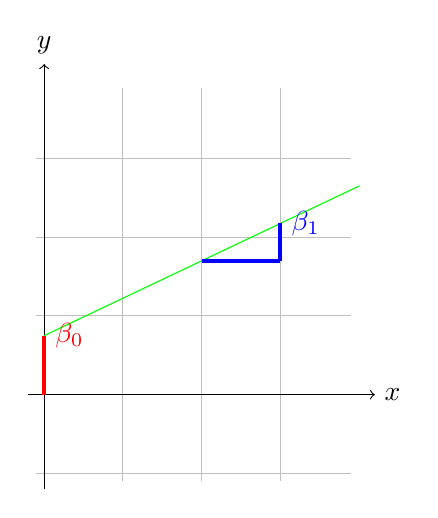
\begin{tikzpicture}[domain=0:4]
            \draw[thin,color=gray!50] (-0.1,-1.1) grid (3.9,3.9);
            \draw[->] (-0.2,0) -- (4.2,0) node[right] {$x$};
            \draw[->] (0,-1.2) -- (0,4.2) node[above] {$y$};
            \draw[domain=0:4, color=green] plot (\x,0.475*\x + 0.75) node[right] {${}$};
            \draw (0,0)--(0,0.75);
            \draw [line width=1.5, red] (0,0)--(0,0.75) node[right] {${\beta _{0}}$}; 
            \draw [line width=1.5, blue] (2,1.7)--(3,1.7) node[left] {${}$}; 
            \draw [line width=1.5, blue] (3,1.7)--(3,2.175) node[right] {${\beta _{1}}$}; 
        \end{tikzpicture}
        
        \textit{Equation of a straight line ${E(Y|X=x)=\beta _{0} + \beta _{1} x}$} 
    \end{center}
    
    In fact, we can not accurately determine the parameter $\beta_{0}$ or $\beta_{1}$ because it is unknown but only estimated by using data. By changing the parameters, we can get all possible straight lines. That is why the general equation we have a certain error. Therefore, we will process and get results from data to the overall estimate. 
	
    The simplest way to explain is to suppose we have a data set with x and y values that make a lot of points on the graph, and through these points, we can plot many linear lines to show the relationship linearity between x and y, but we can only choose \textbf{one} line that best represents of this relationship, corresponding to the fact that we have only make a single linear regression equation.
    
    \pgfplotsset{width=7.5cm,compat=1.12}
    \begin{center}
    \usepgfplotslibrary{fillbetween}
    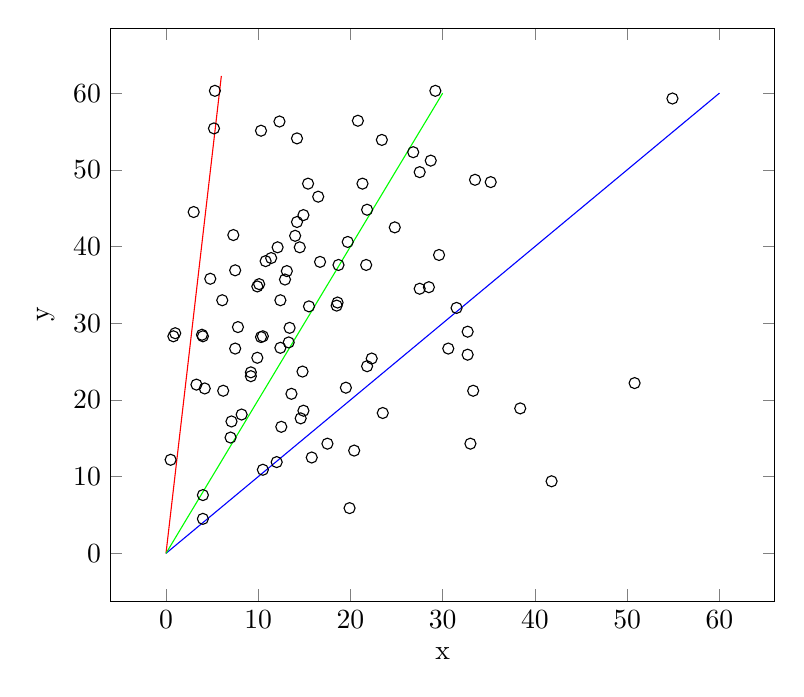
\begin{tikzpicture}
      \pgfplotsset{
          scale only axis,
      }
        
          \begin{axis}[
            title={},
            xlabel=x,
            ylabel=y,
          ]
          
            \addplot [color=red, domain=0:6, mark=none] {0.0051026+10.372231*\x};
            
            \addplot [color=blue, domain=0:60, mark=none] 
            {0.005+1.0*\x};
            
            \addplot [color= green, domain=0:30, mark=none] 
            {0.005+2.0*\x};
            
            \addplot[only marks, mark=o]
            coordinates{ % plot 1 data set
                (3,44.5)(15.8,12.5)(13.1,36.8)(4,7.6)(1,28.7)
                (10.5,28.3)(27.5,49.7)(7,15.1)(28.7,51.2)(19.9,5.9)
                (6.1,33)(14.2,54.1)(10.3,28.2)(41.8,9.4)(0.8,28.3)
                (12,11.9)(33.5,48.7)(12.1,39.9)(17.5,14.3)(23.4,53.9)
                (13.6,20.8)(14.8,23.7)(12.3,56.3)(14,41.4)(10.5,10.9)
                (33,14.3)(18.6,32.7)(12.4,33)(22.3,25.4)(20.4,13.4)
                (10.1,35.1)(9.2,23.6)(12.4,26.8)(3.3,22)(0.5,12.2)
                (12.5,16.5)(15.4,48.2)(19.5,21.6)(13.3,27.5)(3.9,28.5)
                (14.9,18.6)(14.9,44.1)(18.7,37.6)(5.2,55.4)(5.3,60.3)
                (4,4.5)(29.6,38.9)(28.5,34.7)(27.5,34.5)(4.2,21.5)
                (7.5,26.7)(21.8,24.4)(12.9,35.7)(7.1,17.2)(11.4,38.5)
                (16.5,46.5)(14.2,43.2)(4,28.3)(21.8,44.8)(13.4,29.4)
                (7.3,41.5)(16.7,38)(4.8,35.8)(9.9,34.8)(10.8,38.1)
                (6.2,21.2)(9.9,25.5)(30.6,26.7)(9.2,23.1)(19.7,40.6)
                (14.5,39.9)(33.3,21.2)(32.7,25.9)(38.4,18.9)(7.5,36.9)
                (32.7,28.9)(8.2,18.1)(10.3,55.1)(26.8,52.3)(54.9,59.3)
                (7.8,29.5)(14.6,17.6)(21.3,48.2)(35.2,48.4)(15.5,32.2)
                (50.8,22.2)(24.8,42.5)(29.2,60.3)(21.7,37.6)(20.8,56.4)
                (23.5,18.3)(18.5,32.3)(31.5,32)
              % more points...
            }; \label{plot_one}
        
            % plot 1 legend entry
            \addlegendimage{/pgfplots/refstyle=plot_one}
          \end{axis}
    \end{tikzpicture}
    \end{center}
    
    The \textit{variance function} (2) is assumed to be constant, with a positive value ${\sigma ^ {2}}$ that is usually unknown. When ${\sigma ^ {2} > 0}$, the observed value of the ${i^{th}}$ response ${y_{i}}$ will not equal to its expected value ${E(Y|X=x_{i})}$. To explain the difference between the observed data and the expected value, we have to make a quantitative called a statistical error or ${e_{i}}$= ${y_{i}}$ - ${E(Y|X=x_{i})}$. 
    
    The errors ${e_{i}}$ depend on unknown parameters in the mean function and so are not observable quantities.

\section{Statistical Hypotheses}
    If we make assumptions when the chief null hypothesis is ${H_{0}}$: ${B_{1} = 0}$ (i.e the equation ${E(Y|X=x)}$ is parallel to the horizontal axis) and the corresponding alternative hypothesis is ${H_{1}}$: ${B_{1} = 0}$ (i.e the equation ${E(Y|X=x)}$ is not parallel to the horizontal axis or ${H_{1}}$ is negative. by ${H_{0}}$). If ${H_{0}}$ is true, we can conclude that for every variable x, it has no effect on Y. 
    \\
    
    For \textbf{Figure 3.1}, we might expect the straight-line to be appropriate but with ${B_{1} = 0}$. If the slope is zero, then the line is parallel to the horizontal axis. We will test for independence of x and y by testing the hypothesis that ${\beta_{1} = 0}$ against the alternative hypothesis that ${\beta_{1} = 0}$.
    
    \begin{center}
    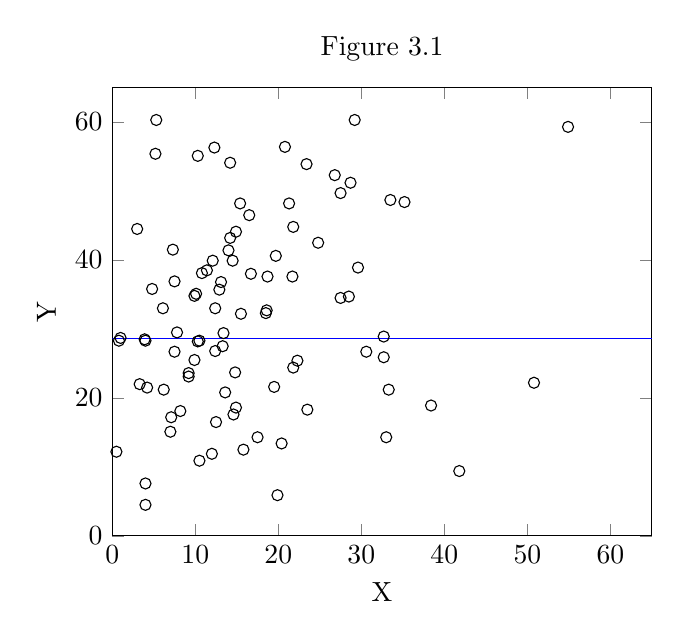
\begin{tikzpicture}
        
        \begin{axis}[
            title={\testbf{Figure 3.1}},
            xlabel={X}, ylabel={Y},
            xmin=0, xmax=65, ymin=0, ymax=65,
            xtick={}, ytick={},
            enlargelimits=false,
        ]
            
        \addplot [color=blue, domain=0:70, mark=none] {28.60+0.0*\x};
            
        \addplot[only marks, mark= o]
        coordinates{ % plot 1 data set
            (3,44.5)
            (15.8,12.5)(13.1,36.8)(4,7.6)
            (1,28.7)(10.5,28.3)(27.5,49.7)
            (7,15.1)(28.7,51.2)(19.9,5.9)
            (6.1,33)(14.2,54.1)(10.3,28.2)
            (41.8,9.4)(0.8,28.3)(12,11.9)
            (33.5,48.7)(12.1,39.9)(17.5,14.3)
            (23.4,53.9)(13.6,20.8)(14.8,23.7)
            (12.3,56.3)(14,41.4)(10.5,10.9)
            (33,14.3)(18.6,32.7)(12.4,33)
            (22.3,25.4)(20.4,13.4)(10.1,35.1)
            (9.2,23.6)(12.4,26.8)(3.3,22)
            (0.5,12.2)(12.5,16.5)(15.4,48.2)
            (19.5,21.6)(13.3,27.5)(3.9,28.5)
            (14.9,18.6)(14.9,44.1)(18.7,37.6)
            (5.2,55.4)(5.3,60.3)(4,4.5)
            (29.6,38.9)(28.5,34.7)(27.5,34.5)
            (4.2,21.5)(7.5,26.7)(21.8,24.4)
            (12.9,35.7)(7.1,17.2)(11.4,38.5)
            (16.5,46.5)(14.2,43.2)(4,28.3)
            (21.8,44.8)(13.4,29.4)(7.3,41.5)
            (16.7,38)(4.8,35.8)(9.9,34.8)
            (10.8,38.1)(6.2,21.2)(9.9,25.5)
            (30.6,26.7)(9.2,23.1)(19.7,40.6)
            (14.5,39.9)(33.3,21.2)(32.7,25.9)
            (38.4,18.9)(7.5,36.9)(32.7,28.9)
            (8.2,18.1)(10.3,55.1)(26.8,52.3)
            (54.9,59.3)(7.8,29.5)(14.6,17.6)
            (21.3,48.2)(35.2,48.4)(15.5,32.2)
            (50.8,22.2)(24.8,42.5)(29.2,60.3)
            (21.7,37.6)(20.8,56.4)(23.5,18.3)
            (18.5,32.3)
          % more points...
        };
        \end{axis}
        
    \end{tikzpicture}
    \end{center}
    
    Sometimes it is reasonable to choose a different null hypothesis for ${B_{1}}$. For example, if ${x}$ is some \textbf{gold standard} for a particular measurement, i.e., a best-quality measurement often involving great expense, and y is some cheaper substitute, then the obvious null hypothesis is ${B_{1} = 1}$ with alternative ${B_{1} != 1}$.
    
    \begin{center}
    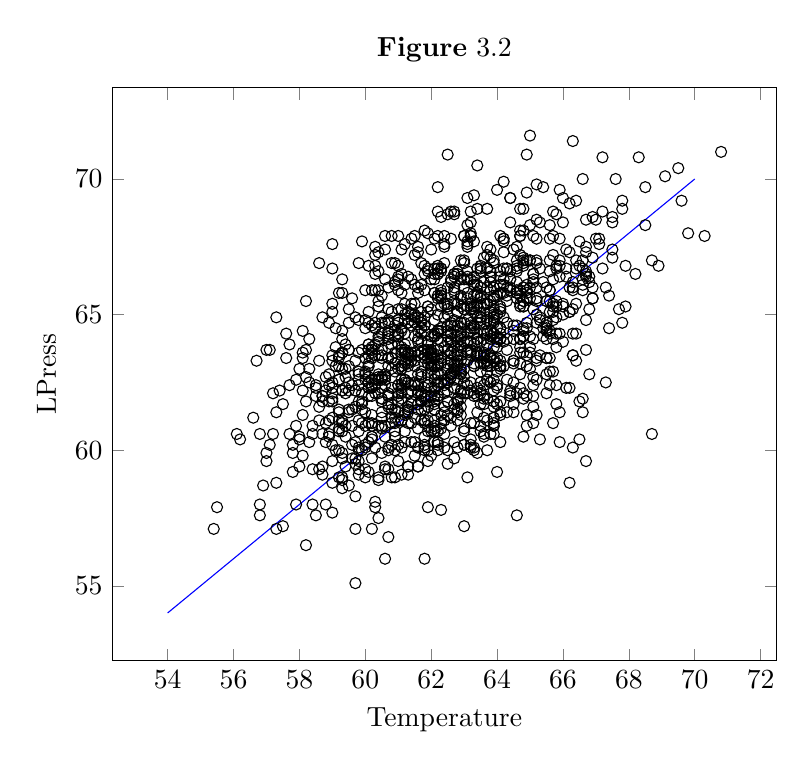
\begin{tikzpicture}
      \pgfplotsset{
          scale only axis,
      }
    
      \begin{axis}[
        title={\textbf{Figure} 3.2},
        xlabel=Temperature,
        ylabel=LPress,
      ]
        \addplot[only marks, mark= o]
        coordinates{ % plot 1 data set
            (59.7,55.1)(58.2,56.5)(60.6,56)(60.7,56.8)
            (61.8,56)(55.5,57.9)(55.4,57.1)(56.8,57.6)(57.5,57.2)
            (57.3,57.1)(58.5,57.6)(59.7,57.1)(59,57.7)(60.4,57.5)
            (60.2,57.1)(60.3,57.9)(61.9,57.9)(62.3,57.8)(63,57.2)
            (64.6,57.6)(56.8,58)(56.9,58.7)(57.9,58)(57.3,58.8)
            (58.8,58)(58.4,58)(59.3,58.6)(59.3,58.9)(59,58.8)
            (59.7,58.3)(59.5,58.7)(60.4,58.9)(60.3,58.1)(66.2,58.8)
            (57,59.6)(57.8,59.2)(57.8,59.9)(57,59.9)(58.6,59.3)
            (58.4,59.3)(58,59.4)(58.7,59.4)(58.7,59.1)(58.1,59.8)
            (59.7,59.7)(59,59.6)(59.2,59)(59.3,59.9)(59.8,59.1)
            (59.7,59.5)(59.6,59.7)(59.3,59)(59.3,59.7)(59.4,59.4)
            (59.8,59.6)(59.8,59.3)(60.4,59)(60.9,59)(60.2,59.7)
            (60.5,59.9)(60,59)(60.6,59.3)(60.7,59.3)(60.8,59)
            (60,59.3)(60.6,59.4)(60.1,59.2)(61.3,59.4)(61.9,59.6)
            (61.1,59.1)(61,59.6)(61.6,59.4)(61.6,59.4)(61.5,59.8)
            (61.3,59.4)(61.3,59.1)(62.5,59.5)(62.7,59.7)(62,59.8)
            (63.1,59)(63.4,59.9)(64,59.2)(66.7,59.6)(56.2,60.4)
            (56.1,60.6)(56.8,60.6)(57.8,60.2)(57.9,60.9)(57.7,60.6)
            (57.2,60.6)(57.1,60.2)(58.4,60.6)(58.9,60.5)(58.7,60.6)
            (58,60.5)(58.8,60.3)(58.4,60.9)(58,60.4)(58.9,60.6)
            (58.3,60.3)(59,60.2)(59.6,60.9)(59.8,60)(59.4,60.5)
            (59.2,60.8)(59.6,60.2)(59.3,60.7)(59.4,60.9)(59.8,60.1)
            (59.9,60)(59.8,60.7)(59.2,60.7)(59.2,60)(59.7,60.3)
            (59.1,60)(60.5,60.8)(60.2,60.5)(60.2,60.4)(60,60.9)
            (60.3,60.1)(60.5,60.9)(60.4,60.9)(60.6,60.9)(60.7,60)
            (60.2,60.9)(60.6,60.5)(60.2,60.5)(60.9,60)(60.7,60.1)
            (60,60.2)(60,60.1)(60.8,60.2)(60.1,60.3)(60.9,60.7)
            (60.9,60.5)(61.2,60.3)(61.8,60.2)(61.2,60.7)(61.9,60)
            (61.6,60.1)(61.8,60.5)(61.6,60.8)(61,60.2)(61.5,60.3)
            (61.4,60.3)(61.9,60.9)(61.9,60.7)(61.1,60.1)(61.8,60)
            (61.8,60.1)(61.6,60.1)(62.2,60.2)(62.4,60.6)(62.2,60)
            (62.1,60.9)(62.3,60.8)(62.4,60.1)(62.1,60.8)(62.1,60.3)
            (62.8,60.1)(62.2,60.3)(62.1,60.7)(62.2,60.7)(62,60.7)
            (62.7,60.3)(62.5,60)(62.2,60.3)(62.6,60.9)(63.5,60.9)
            (63.3,60)(63.8,60.6)(63.6,60.5)(63.7,60)(63.2,60.1)
            (63.5,60.7)(63,60.2)(63.3,60.1)(63.2,60.2)(63,60.7)
            (63,60.8)(63.6,60.6)(63.2,60.4)(63.9,60.6)(63.9,60.9)
            (63,60.2)(63.9,60.9)(64.1,60.3)(64.9,60.9)(64.8,60.5)
            (65.3,60.4)(65.9,60.3)(66.3,60.1)(66.5,60.4)(68.7,60.6)
            (56.6,61.2)(57.5,61.7)(57.3,61.4)(58.6,61.6)(58.2,61.8)
            (58.1,61.3)(58.7,61.8)(58.8,61)(58.9,61.1)(58.9,61.8)
            (58.6,61.1)(59.9,61.7)(59.2,61.4)(59.8,61.8)(59.6,61.5)
            (59,61.2)(59.9,61)(59,61.9)(59.8,61.1)(59.9,61.8)
            (59.9,61.5)(59,61.8)(59.5,61.4)(59.7,61.6)(59.5,61.5)
            (59.3,61.1)(59.2,61.1)(59.3,61)(59.2,61.5)(60,61.4)
            (60.5,61.9)(60.7,61.6)(60.5,61.8)(60.1,61)(60.2,61.3)
            (60.8,61)(60.5,61.4)(60.9,61.2)(60.5,61.9)(60.9,61.5)
            (60.8,61.5)(60.9,61)(60.7,61.7)(60.5,61.2)(60.8,61.7)
            (60.2,61)(60.8,61.2)(61.4,61)(61.9,61.6)(61.7,61.8)
            (61.8,61.9)(61.7,61.5)(61.3,61.4)(61,61.8)(61.8,61)
            (61.7,61.1)(61.2,61.4)(61.6,61.7)(61.9,61.6)(61.9,61.8)
            (61.3,61.6)(61.6,61.5)(61.5,61.2)(61.8,61.5)(61.8,61.1)
            (61,61.4)(61.6,61.7)(61.3,61.6)(61.4,61.7)(61.3,61.5)
            (61.1,61.9)(61.7,61.8)(61.1,61.1)(61.3,61.5)(61.2,61.3)
            (61.3,61)(61.9,61.1)(61.7,61.8)(61,61.1)(61.1,61.1)
            (61.4,61.8)(62.4,61.6)(62.8,61.1)(62.5,61.8)(62.1,61.1)
            (62.8,61.5)(62.8,61.8)(62.1,61.7)(62.8,61.9)(62.1,61.5)
            (62.5,61.3)(62.8,61.8)(62.8,61.4)(62.3,61)(62.3,61.3)
            (62.7,61.5)(62.7,61.7)(62.9,61.9)(62.4,61.4)(62.6,61.2)
            (62.9,61.6)(62.5,61.8)(62.4,61.1)(62.1,61.5)(62.2,61.9)
            (62.4,61.1)(62.9,61.3)(62.1,61.8)(63.3,61)(63.9,61.2)
            (63.9,61.8)(63.9,61.6)(63.9,61)(63.6,61.7)(63.9,61.2)
            (63.5,61.7)(63.6,61.9)(63.7,61.1)(63.2,61)(63.6,61.2)
            (63.4,61.4)(63.9,61.8)(63.7,61.9)(64.9,61.3)(64.5,61.7)
            (64,61.7)(64.1,61.8)(64.1,61.3)(64.8,61.9)(64.3,61.4)
            (64.1,61.4)(64.5,61.4)(65.8,61.7)(65.7,61)(65.2,61.3)
            (65.1,61.6)(65.1,61)(65.9,61.4)(66.5,61.8)(66.6,61.9)
            (66.6,61.4)(57.4,62.2)(57.2,62.1)(57.7,62.4)(57.9,62.6)
            (58.3,62.5)(58.5,62)(58.8,62.7)(58.1,62.2)(58.8,62.2)
            (58.5,62.4)(58.7,62)(58.9,62.8)(58.5,62.3)(58.9,62.4)
            (58.2,62.7)(58.7,62)(59.9,62.1)(59.8,62.8)(59.7,62.2)
            (59.4,62.1)(59.2,62.6)(59.3,62.2)(59,62.5)(59.2,62.6)
            (59.7,62.2)(59.5,62.2)(59.6,62.4)(59,62.1)(59.4,62.3)
            (59.5,62.5)(59.3,62.2)(59,62.3)(59.8,62.9)(59.8,62.4)
            (59.4,62.7)(59.8,62.6)(60.3,62.6)(60.5,62.6)(60.6,62.6)
            (60.1,62.5)(60.2,62.4)(60.1,62.7)(60.2,62)(60.1,62)
            (60.7,62)(60.3,62.1)(60.9,62.9)(60.7,62)(60.8,62.3)
            (60.5,62.7)(60.1,62.3)(60.2,62.3)(60.4,62.6)(60.6,62.8)
            (60.4,62.1)(60.4,62.8)(60.1,62.3)(60,62.8)(60.5,62.3)
            (60.3,62.4)(60.6,62.7)(60.2,62.6)(60.5,62.7)(60.4,62.7)
            (60.7,62.1)(60.6,62.4)(60.1,62.5)(60,62.6)(60,62.9)
            (61.7,62)(61.8,62)(61.2,62.5)(61.6,62.8)(61.5,62.4)
            (61.1,62.4)(61.9,62.5)(61.2,62.6)(61.7,62.7)(61.6,62.2)
            (61.5,62.5)(61.2,62.6)(61.4,62.4)(61.1,62.2)(61,62.4)
            (61.3,62.1)(61.6,62.1)(61,62)(61.7,62.1)(61.8,62.3)
            (61.7,62.9)(61.3,62.5)(61.4,62.2)(61.1,62.1)(61,62.1)
            (61.3,62.5)(61.6,62.4)(61.9,62.8)(61,62.4)(61.1,62.6)
            (61.9,62.4)(61.1,62.3)(61.7,62.1)(61.3,62.1)(61.7,62.8)
            (62,62.3)(62.6,62.7)(62.1,62.2)(62,62)(62.5,62.5)
            (62.6,62.8)(62.2,62.4)(62.9,62.8)(62.5,62.2)(62.9,62.9)
            (62.2,62)(62.8,62.6)(62.2,62.8)(62.5,62.5)(62.4,62.4)
            (62.3,62.8)(62.1,62.6)(62.7,62.3)(62.5,62.6)(62.4,62.1)
            (62.4,62.6)(62.9,62.8)(62.2,62.5)(62.1,62)(62.9,62.1)
            (62.6,62.7)(62.6,62.8)(62.7,62.3)(62.1,62.3)(62.3,62.5)
            (62.1,62.8)(62.9,62.2)(62.6,62.8)(62.7,62.9)(62.7,62.6)
            (63.2,62.2)(63.7,62.6)(63.9,62.6)(63,62.7)(63.3,62)
            (63.9,62.2)(63.6,62.4)(63.7,62.6)(63.8,62.5)(63.1,62.4)
            (63.1,62.1)(63.3,62.1)(63.4,62.3)(63,62.1)(63.5,62.9)
            (63.7,62.9)(63.4,62)(63.6,62)(63.8,62.5)(63.5,62.2)
            (63.5,62.1)(63.2,62.5)(63,62.5)(63.5,62.5)(64.9,62)
            (64.4,62)(64.4,62.2)(64.3,62.6)(64.7,62.8)(64.5,62.5)
            (64.8,62.1)(64,62.4)(64,62.9)(64.7,62.3)(64.4,62.1)
            (64,62.3)(64.6,62.1)(65.2,62.6)(65.1,62.4)(65.1,62.7)
            (65.5,62.1)(65.8,62.4)(65.7,62.9)(65.6,62.9)(65.5,62.8)
            (65.6,62.4)(65.1,62)(66.1,62.3)(66.2,62.3)(66.8,62.8)
            (67.3,62.5)(56.7,63.3)(57.7,63.9)(57.6,63.4)(57,63.7)
            (57.1,63.7)(58,63)(58.2,63.7)(58.6,63.3)(58.1,63.6)
            (58.1,63.4)(58.3,63)(59.5,63.7)(59.3,63)(59.9,63.7)
            (59,63.3)(59.5,63.1)(59.1,63.8)(59.3,63.6)(59.7,63.3)
            (59.1,63.1)(59.3,63.6)(59.5,63.7)(59.2,63.4)(59.4,63)
            (59,63.5)(59.2,63.1)(59.4,63.9)(59.2,63.5)(59.8,63.6)
            (60.5,63.7)(60.7,63.4)(60.8,63)(60.2,63.8)(60.1,63.9)
            (60.2,63.7)(60.9,63.2)(60.5,63.4)(60.5,63.5)(60.2,63.6)
            (60,63.4)(60.1,63.2)(60.7,63.8)(60.1,63.1)(60.7,63.1)
            (60.7,63.4)(60.3,63.9)(60.3,63.5)(60.1,63.1)(60.8,63.9)
            (60.9,63.2)(60.4,63.5)(60.8,63.4)(60.1,63.5)(60.2,63.4)
            (60.1,63.9)(60.1,63.7)(60.9,63.6)(60.8,63.4)(61.9,63.2)
            (61.2,63.2)(61.1,63.1)(61.5,63.6)(61.6,63.5)(61.1,63)
            (61.3,63.1)(61.2,63.3)(61.4,63.3)(61.4,63.6)(61.6,63.7)
            (61.1,63.1)(61.9,63.4)(61.7,63.6)(61,63)(61.1,63.1)
            (61.8,63.5)(61.2,63.9)(61.1,63.6)(61.3,63.5)(61.1,63.7)
            (61.2,63.7)(61.9,63.2)(61.2,63.6)(61.9,63.9)(61.1,63)
            (61.2,63.6)(61.5,63.3)(61.3,63.6)(61.1,63.8)(61.3,63.2)
            (61.4,63.5)(61.9,63.7)(61,63.9)(61.5,63.1)(61.3,63.4)
            (61.4,63.3)(61.8,63.4)(61.8,63.7)(61.9,63.6)(61.6,63.5)
            (61.2,63.7)(62.7,63.1)(62.6,63.6)(62.3,63.4)(62.8,63.5)
            (62.1,63.1)(62.9,63.5)(62.1,63.4)(62.4,63.8)(62.5,63)
            (62.6,63.6)(62,63.6)(62.2,63.5)(62,63.6)(62.8,63.7)
            (62.8,63.3)(62,63.6)(62,63.4)(62.2,63.7)(62.8,63.2)
            (62.1,63.1)(62,63)(62.5,63.2)(62.2,63.2)(62.9,63.3)
            (62.7,63)(62.5,63.5)(62.7,63.5)(62.3,63.3)(62,63.1)
            (62.6,63.3)(62.7,63.8)(62,63.2)(62.3,63.2)(62,63.6)
            (62.5,63.7)(62.9,63)(62,63.3)(62.9,63.9)(62,63.5)
            (62.9,63.8)(62.2,63.7)(62.2,63.1)(62,63.7)(62.7,63.2)
            (62.1,63.5)(62.8,63.1)(63.5,63.5)(63.3,63.2)(63.5,63.2)
            (63.8,63.5)(63.2,63.6)(63.4,63.6)(63.6,63.6)(63.6,63.4)
            (63.7,63.3)(63.2,63.7)(63.6,63.5)(63.7,63.9)(63.7,63.3)
            (63,63)(63.8,63.1)(63.3,63.9)(63.9,63.8)(63.6,63.5)
            (63.1,63.6)(63.9,63.3)(63.8,63.5)(63.8,63.4)(63.2,63.5)
            (63.5,63.5)(63.6,63.2)(63.3,63.1)(63.7,63.2)(63.1,63.7)
            (63.1,63.3)(63.7,63.1)(63.4,63.6)(63.9,63.4)(63.3,63.1)
            (63.4,63.5)(64.1,63.1)(64,63.2)(64.8,63.6)(64.7,63.2)
            (64.2,63.1)(64.5,63.3)(64.7,63.8)(64.5,63.3)(64.7,63.6)
            (64,63.8)(64.9,63.5)(64.1,63)(64.9,63.1)(64.5,63.2)
            (64,63.4)(64.1,63.1)(64.3,63.7)(64.1,63.3)(65.5,63.4)
            (65,63)(65.2,63.3)(65.5,63.4)(65,63.8)(65.3,63.5)
            (65.6,63.4)(65.2,63.4)(65,63.6)(65.8,63.8)(66.7,63.7)
            (66.3,63.5)(66.4,63.3)(66.3,63.5)(57.6,64.3)(57.3,64.9)
            (58.1,64.4)(58.3,64.1)(58.9,64.7)(58.7,64.9)(59.3,64.4)
            (59.5,64.7)(59.8,64.8)(59.1,64.5)(59.3,64.1)(59.7,64.9)
            (60.7,64.3)(60.7,64.1)(60.9,64.4)(60.7,64.2)(60.4,64.2)
            (60.1,64.7)(60.2,64.6)(60.3,64.7)(60.7,64.4)(60.9,64.6)
            (60.4,64.1)(60.7,64.7)(60.5,64.3)(60.6,64.7)(60,64.8)
            (60.3,64.5)(60.4,64)(60,64.5)(60.9,64.2)(60.5,64.7)
            (60.7,64.3)(60.3,64.5)(60.7,64.8)(60.5,64.9)(61.6,64.4)
            (61,64.3)(61.7,64.3)(61.6,64.9)(61.6,64.1)(61.7,64.7)
            (61.6,64)(61.6,64.9)(61.8,64.6)(61.8,64.4)(61.3,64.7)
            (61.7,64)(61.2,64.8)(61,64.8)(61.8,64.9)(61.7,64.5)
            (61.2,64.3)(61.5,64.7)(61,64.8)(61.4,64.8)(61,64.7)
            (61.7,64.8)(61,64.3)(61.5,64.9)(61.3,64.7)(61,64.2)
            (61.1,64.4)(61.1,64.5)(61.8,64.6)(61.4,64.6)(61.5,64.2)
            (61.9,64)(62.6,64.7)(62.2,64.1)(62.9,64.3)(62.9,64.2)
            (62.6,64.3)(62.3,64)(62.9,64.1)(62.8,64.6)(62.6,64.1)
            (62.2,64.4)(62.8,64.2)(62.1,64.2)(62.6,64)(62.1,64.8)
            (62.6,64.3)(62.2,64.4)(62.2,64.4)(62.7,64.6)(62.8,64)
            (62.9,64.5)(62,64.2)(62.3,64.5)(62.6,64.3)(62.9,64.7)
            (62.9,64.7)(62.5,64)(62.1,64.2)(62.2,64.3)(62.6,64.6)
            (62.5,64.2)(62.4,64.9)(62.8,64)(62.7,64.8)(62.8,64.4)
            (62.3,64.4)(62.5,64.6)(62.5,64.4)(62.1,64.3)(63.2,64)
            (63.4,64.7)(63.4,64.1)(63.8,64.7)(63.9,64.3)(63.3,64.3)
            (63.5,64.7)(63,64.7)(63.9,64.9)(63.9,64.7)(63.8,64.2)
            (63.2,64.4)(63.8,64.1)(63.9,64.9)(63.3,64.6)(63.9,64.3)
            (63.2,64.7)(63.6,64.3)(63.6,64.1)(63.4,64.9)(63.7,64.4)
            (63,64)(63.5,64.9)(63.4,64.1)(63.1,64.8)(63.1,64)
            (63.2,64.6)(63.8,64.4)(63.2,64.5)(63.3,64.5)(63.7,64.8)
            (63.5,64)(63.7,64.3)(63.9,64.3)(63.7,64.9)(63.5,64.9)
            (63.4,64)(63.5,64.8)(63.9,64.8)(63.1,64.3)(64.5,64.6)
            (64.1,64.1)(64.1,64.1)(64.5,64.4)(64.7,64.1)(64.6,64.6)
            (64.8,64.4)(64.7,64.1)(64,64.2)(64.1,64.1)(64.1,64.5)
            (64.1,64.3)(64.2,64.9)(64.3,64.7)(64.1,64.5)(64.8,64.2)
            (64.7,64.1)(64.9,64.5)(64.8,64.2)(64.8,64.5)(64.2,64)
            (64,64.1)(64.8,64.2)(64.9,64.7)(64,64)(64.5,64.1)
            (64.3,64.1)(64,64.5)(65.9,64.3)(65.3,64.9)(65.7,64.1)
            (65.6,64.3)(65,64.2)(65.8,64.9)(65.7,64.8)(65.5,64.4)
            (65.5,64.6)(65.5,64.1)(65.8,64.3)(65.3,64.8)(65.2,64.7)
            (65.5,64.7)(65.4,64.5)(65.6,64.4)(65.1,64.1)(65.5,64.5)
            (65.4,64.2)(66.7,64.8)(66,64)(66.3,64.3)(66.4,64.3)
            (67.4,64.5)(67.8,64.7)(58.2,65.5)(59.6,65.6)(59.3,65.8)
            (59.5,65.2)(59.2,65.8)(59,65.4)(59,65.1)(60,65.9)
            (60.4,65.3)(60.7,65.2)(60.2,65.9)(60.8,65.1)(60.1,65.1)
            (60.4,65.9)(60.3,65.9)(60.4,65.5)(60.5,65.7)(61.7,65.1)
            (61.2,65)(61.4,65.2)(61.9,65.3)(61.5,65.4)(61.9,65.3)
            (61.4,65.4)(61.2,65.4)(61.3,65.1)(61.4,65)(61.8,65.9)
            (61.6,65.8)(61.1,65.2)(61.5,65)(61.1,65.8)(61,65.9)
            (61,65.2)(61.9,65.1)(62.8,65.1)(62.5,65.3)(62.5,65)
            (62.9,65.3)(62.7,65.4)(62.5,65.2)(62.7,65.9)(62.3,65.6)
            (62.3,65.7)(62.3,65.8)(62.9,65.7)(62.8,65.4)(62.2,65)
            (62.7,65.8)(62.5,65.4)(62.2,65.6)(62.5,65.3)(62.1,65.8)
            (62.3,65.7)(62.1,65.8)(62.4,65.4)(62.2,65.7)(62.3,65.9)
            (62.7,65.5)(62.8,65.1)(62,65.2)(62.9,65.6)(62.3,65.3)
            (63.1,65.8)(63.8,65.1)(63.9,65.6)(63.3,65.7)(63.4,65.4)
            (63.4,65.8)(63.8,65.1)(63.4,65.7)(63.7,65.4)(63.4,65.7)
            (63.9,65.7)(63.2,65.4)(63.7,65.4)(63.8,65.9)(63.9,65.3)
            (63.3,65.2)(63.9,65.2)(63.5,65.6)(63.5,65.3)(63.1,65.3)
            (63.1,65.6)(63.8,65.5)(63.6,65.4)(63.2,65.3)(63.5,65.6)
            (63.3,65.3)(63.9,65)(63.9,65.6)(63.4,65.3)(63.5,65.7)
            (63.3,65.1)(63.2,65.2)(63.7,65.4)(63,65.2)(63,65.2)
            (64.1,65.3)(64.6,65.8)(64.7,65.9)(64,65)(64.2,65.8)
            (64.6,65.8)(64.6,65.6)(64.9,65.9)(64.6,65.8)(64.8,65.3)
            (64.1,65.2)(64.1,65.8)(64.7,65.4)(64.6,65.9)(64.9,65.8)
            (64.7,65.7)(64.8,65.5)(64.7,65.3)(64.8,65.3)(64.4,65.9)
            (64.8,65.5)(64.1,65.1)(64.3,65.7)(64.9,65.6)(64,65.7)
            (64.3,65.5)(65.6,65.9)(65.2,65.6)(65.2,65.5)(65.8,65.3)
            (65.8,65.5)(65.5,65.5)(65.7,65.3)(65.7,65.4)(65.2,65)
            (65.7,65.1)(65.1,65.2)(65.6,65.1)(65.6,65.5)(65.6,65.9)
            (65,65.6)(65.5,65.5)(66.2,65.1)(66.9,65.6)(66,65.3)
            (66,65)(66,65.4)(66.2,65.1)(66.4,65.4)(66.8,65.2)
            (66.9,65.6)(66.3,65.2)(66.6,65.9)(66.3,65.9)(67.7,65.2)
            (67.4,65.7)(67.9,65.3)(58.6,66.9)(59.3,66.3)(59,66.7)
            (59.8,66.9)(60.3,66.8)(60.9,66.9)(60.1,66.8)(60.3,66.5)
            (60.4,66.6)(60.7,66)(60.9,66.1)(60.9,66.2)(60.8,66.9)
            (60.6,66.3)(61.2,66.1)(61,66.8)(61,66.3)(61.8,66.5)
            (61.4,66.3)(61.7,66.1)(61.8,66.8)(61.6,66)(61.5,66.1)
            (61,66.4)(61.3,66.4)(61.9,66.6)(61.1,66.5)(61.7,66.9)
            (61.9,66.7)(62.7,66.5)(62.2,66.7)(62,66.3)(62.5,66)
            (62.8,66.6)(62.3,66.7)(62.2,66.8)(62.3,66.6)(62.1,66.5)
            (62.6,66.3)(62.1,66.3)(62.4,66.9)(62.3,66.7)(62.2,66.5)
            (62.9,66.3)(62.7,66)(62.1,66.7)(62.8,66.5)(62.7,66.5)
            (62.6,66.2)(62.2,66.5)(62.7,66.4)(62.9,66.4)(63.8,66.2)
            (63.1,66.6)(63.1,66.3)(63.7,66.7)(63,66.3)(63.5,66)
            (63.5,66.7)(63.8,66.4)(63.6,66.2)(63.8,66.2)(63.9,66)
            (63.4,66.1)(63.3,66.4)(63.1,66.4)(63.9,66.9)(63.7,66.7)
            (63,66)(63.2,66.3)(63.8,66.4)(63.5,66.8)(63.9,66)
            (63.3,66.2)(63.8,66.6)(63.4,66.7)(63.3,66.1)(63.5,66)
            (63,66.9)(63.5,66.6)(63.7,66)(64.8,66.9)(64.8,66)
            (64.8,66)(64.6,66.7)(64.1,66.1)(64.1,66.6)(64.3,66.7)
            (64.4,66.3)(64.3,66)(64.4,66.6)(64.8,66.8)(64.2,66.1)
            (64.6,66.6)(64.2,66.7)(64.6,66.2)(64.4,66)(64.6,66.8)
            (64.2,66.3)(64.3,66.7)(64.4,66.3)(64.9,66.1)(64.1,66.4)
            (65.7,66.3)(65,66)(65.8,66.8)(65.4,66.2)(65.9,66.4)
            (65.6,66.6)(65.1,66.3)(65.2,66)(65.9,66.8)(65.3,66.7)
            (65.1,66.5)(65.8,66.7)(65.1,66.5)(65.1,66.2)(65.2,66.9)
            (65.5,66)(66.8,66.4)(66.7,66.4)(66.1,66.4)(66.3,66)
            (66.7,66.6)(66.6,66.3)(66.7,66.5)(66.9,66)(66.6,66.7)
            (66.1,66.7)(66.2,66)(66.5,66.8)(66.3,66.2)(66.6,66.1)
            (66.8,66.2)(66.4,66.7)(67.3,66)(67.2,66.7)(67.9,66.8)
            (68.9,66.8)(68.2,66.5)(59.9,67.7)(59,67.6)(60.6,67.4)
            (60.4,67.3)(60.3,67.5)(60.6,67.9)(60.3,67.2)(60.8,67.9)
            (61.6,67.3)(61.4,67.8)(61,67.9)(61.2,67.6)(61.5,67.2)
            (61.5,67.9)(61.1,67.4)(61.6,67.5)(62.1,67.8)(62.6,67.8)
            (62.2,67.9)(62.4,67.6)(62.4,67.9)(62.9,67)(62.4,67.5)
            (62,67.4)(63.9,67)(63.6,67.1)(63.1,67.7)(63.8,67.4)
            (63,67.9)(63.7,67.5)(63,67.9)(63.8,67.1)(63.3,67.7)
            (63.7,67.2)(63.1,67.5)(63.2,67.9)(63,67)(63.1,67.6)
            (63.2,67.9)(64.2,67.8)(64.7,67.9)(64.5,67.4)(64.8,67)
            (64.9,67)(64.2,67.3)(64.6,67)(64.7,67.2)(64.2,67.8)
            (64.8,67.1)(64.2,67.7)(64.7,67.9)(64.1,67.9)(64.6,67.5)
            (65.6,67.8)(65.6,67)(65.9,67)(65.7,67.2)(65.7,67.9)
            (65.9,67.8)(65.1,67.9)(65.2,67)(65,67)(65.2,67.8)
            (65,67)(66.6,67)(66.7,67.5)(66.9,67.1)(66.5,67.7)
            (66.2,67.3)(66.7,67.3)(66.1,67.4)(66.4,67)(67,67.8)
            (67.1,67.8)(67.1,67.6)(67.5,67.1)(67.5,67.4)(68.7,67)
            (70.3,67.9)(61.9,68)(61.8,68.1)(62.3,68.6)(62.6,68.8)
            (62.7,68.7)(62.5,68.7)(62.7,68.8)(62.2,68.8)(63.2,68.4)
            (63.4,68.9)(63.2,68)(63.1,68.3)(63.7,68.9)(63.2,68.8)
            (64.4,68.4)(64.7,68.9)(64.8,68.9)(64.7,68.1)(64.8,68.1)
            (65.3,68.4)(65,68.3)(65.7,68.8)(65.8,68.7)(65.2,68.5)
            (65.6,68.3)(66,68.4)(66.7,68.5)(66.9,68.6)(67,68.5)
            (67.5,68.4)(67.2,68.8)(67.5,68.6)(67.8,68.9)(68.5,68.3)
            (69.8,68)(62.2,69.7)(63.1,69.3)(63.3,69.4)(64,69.6)
            (64.4,69.3)(64.2,69.9)(64.9,69.5)(64.4,69.3)(65.2,69.8)
            (65.9,69.6)(65.4,69.7)(66.2,69.1)(66,69.3)(66.4,69.2)
            (67.8,69.2)(68.5,69.7)(69.6,69.2)(62.5,70.9)(63.4,70.5)
            (64.9,70.9)(66.6,70)(67.2,70.8)(67.6,70)(68.3,70.8)
            (69.5,70.4)(69.1,70.1)(65,71.6)(66.3,71.4)(70.8,71)
          % more points...
        }; \label{plot_one}
        
        \addplot [color=blue, domain=54:70, mark=none] {0+1*\x};
        
        % plot 1 legend entry
        \addlegendimage{/pgfplots/refstyle=plot_one}
      \end{axis}
    
    \end{tikzpicture}
    \end{center}
    
    For Figure 3.2, which the blue line we assume the parameter ${\beta _{0} = 0}$ and ${\beta _{1} = 1}$
    
\section{Simple linear regression} 

    \begin{center}
        \textbf{Table 4.1: Forbes’ 1857 Data on Boiling Point and Barometric Pressure for 17 Locations in the Alps and Scotland}
        
        \begin{tabular}{|cccc|}
            \hline 
            Case & Temp(F) & Pressure (Inches Hg) & ${Lpres=100log(Pressure)}$ \\
            \hline
            1 & 194.5 & 20.79 & 131.79 \\
            2 & 194.3 & 20.79 & 131.79 \\
            3 & 197.9 & 22.40 & 135.02 \\
            4 & 198.4 & 22.67 & 135.55 \\
            5 & 199.4 & 23.15 & 136.46 \\ 
            6 & 199.9 & 23.35 & 136.83 \\
            7 & 200.9 & 23.89 & 137.82 \\
            8 & 201.1 & 23.99 & 138.00 \\ 
            9 & 201.4 & 24.02 & 138.06 \\
            10 & 201.3 & 24.01 & 138.04 \\
            11 & 203.6 & 25.14 & 140.04 \\
            12 & 204.6 & 26.57 & 142.44 \\
            13 & 209.5 & 28.49 & 145.47 \\
            14 & 208.6 & 27.76 & 144.34 \\
            15 & 210.7 & 29.04 & 146.30 \\
            16 & 211.9 & 29.88 & 147.54 \\
            17 & 212.2 & 30.06 & 147.80 \\
            \hline
        \end{tabular}
    \end{center}
    
    Forbes’ data were collected at $17$ selected locations.
    
\section{Regression calculation} 
    There are many methods for obtaining estimates of parameters in a model. The method we are discussing here is called ordinary least squares (or OLS), in which parameter estimates are chosen to minimize a quantity called \textit{\textbf{the residual sum of squares (RSS)}}.
    
    The table 5.1 will show all formulas that we use to calculate the two parameters: ${\beta_{0}}$ and ${\beta_{1}}$
    
    \begin{center}
        \textbf{Table 5.1: Definitions of Symbols}
        \begin{tabular}{|c|c|c|}
            \hline 
            Quantity & Definition & Description\\ 
            \hline 
            $\overline{x}$ & ${\displaystyle \sum \left(\dfrac{x_{i}}{n}\right)}$ & Average of x \\  
            \hline 
            $\overline{y}$ & ${\displaystyle \sum \left(\dfrac{y_{i}}{n}\right)}$ & Average of y \\
            \hline 
            SXX & ${\displaystyle \sum {\left(x_{i} - \overline{x}\right)}^2}$ & Sum of squares for x \\
            \hline 
            SYY & ${\displaystyle \sum {\left(y_{i} - \overline{y}\right)}^2}$ & Sum of squares for y \\
            \hline
            SXY & ${\displaystyle \sum (x_{i} - \overline{x})(y_{i} - \overline{y})}$ & Sum of cross-products \\
            \hline
            ${SD_{x}}$ & ${\sqrt{\frac{SXX}{n - 1}}}$ & Sample standard deviation of x’s \\
            \hline 
            ${SD_{y}}$ & ${\sqrt{\frac{SYY}{n - 1}}}$ & Sample standard deviation of y’s \\
            \hline 
            ${s_{xy}}$ & ${\dfrac{SXY}{n - 1}}$ & Sample covariance \\ 
            \hline 
            ${r_{xy}}$ & ${\dfrac{s_{xy}}{SD_{x} SD_{y}}}$ & Sample correlation \\ 
            \hline
        \end{tabular}
        
        \vspace{\baselineskip}
        The symbol ${\Sigma}$ means to add all the values or pairs of values in the data. 
    \end{center}
    
    The criterion function for obtaining estimates is based on the residuals. The residuals reflect the inherent asymmetry in the roles of the response and the predictor in regression problems.
    
    \begin{center}
        \pgfplotsset{compat=newest}
        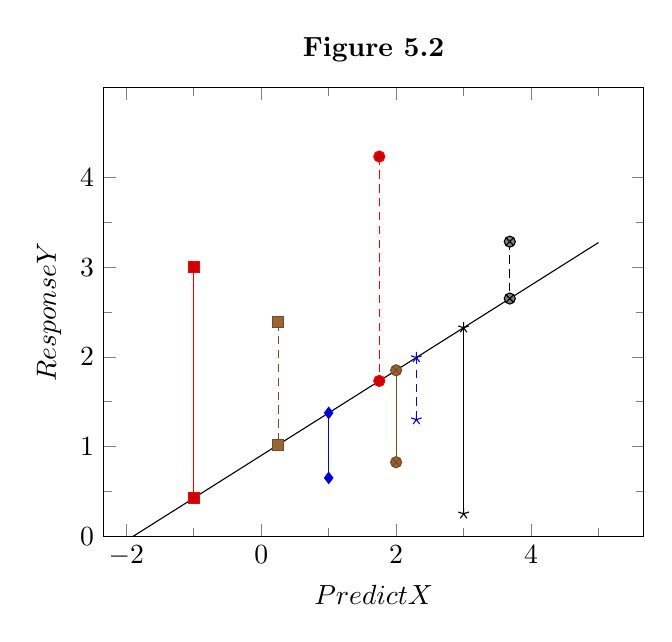
\begin{tikzpicture}
            \begin{axis}[
                title={\textbf{Figure 5.2}},
                xlabel=$Predict X$,		 
                ylabel={$Response Y$},
                minor x tick num={1}, 		
                minor y tick num={1},
                ymin = 0, ymax=5,		 
                ytick={0,1,2,3,4},
            ]
            \addplot[color=black, mark=]{0.475*x + 0.9};
            \addplot coordinates {(-1,0.425) (-1,3)};
	        \addplot coordinates {(2,0.825) (2,1.85)};
	        \addplot coordinates {(3,0.25) (3,2.325)};
	        \addplot coordinates {(1,0.65) (1,1.375)};
	        \addplot coordinates {(1.75,4.234) (1.75,1.73125)};
	        \addplot coordinates {(0.25,2.385) (0.25,1.01875)};
	        \addplot coordinates {(3.685,3.285) (3.685,2.650375)};
	        \addplot coordinates {(2.3,1.3) (2.3,1.9925)};
            \end{axis}
        \end{tikzpicture}
        
        \textit{A schematic plot for OLS fitting. Each data point is indicated by a small symbol. Points below the line have negative residuals, while points above the line have positive residuals.}
    \end{center}
    
    The OLS estimates are those values ${\beta_{0}}$ and ${\beta_{1}}$ that minimize the function. We call the quantity RSS${ \left (\hat{\beta}_{0},{\hat{\beta}_{1}} \right)}$ the \textit{residual sum of squares} or just RSS.
    
    \begin{align}
        RSS(\beta_{0}, \beta_{1}) = \displaystyle \sum _{i = 1} ^ {N}   |y_{i} - (\beta_{0} + \beta_{1} x_{i})| ^ 2
     \end{align}
    
    One of method to find the minimum is differentiate with respect to $\beta_{0}$ and $\beta_{1}$, and make them equal $0$. 
     
    \begin{align} 
        \dfrac{\partial RSS(\beta_{0}, \beta_{1}) }{\beta_{0}} = -2 \displaystyle \sum _{i=1}^{n}  (y_{i} - \beta_{0} - \beta_{1} x_{i}) = 0
        \\
        \dfrac{\partial RSS(\beta_{0}, \beta_{1}) }{\beta_{1}} = -2 \displaystyle \sum _{i=1}^{n}  x_{i} (y_{i} - \beta_{0} - \beta_{1} x_{i}) = 0
    \end{align}
        
    From (11), (12) we get (13) and (14) like this: 
    
    \begin{align} 
        \beta_{0} n + \beta_{1} \displaystyle \sum x_{i} = \displaystyle \sum y_{i}
        \\
        \beta_{0} \displaystyle \sum x_{i} + \beta_{1} \displaystyle \sum x_{i}^2 = \displaystyle \sum x_{i} y_{i}
    \end{align}
    
    Using fomulars: 
    
     \begin{align} 
        SXX &= \Sigma (x_{i} - \overline{x})^2 \\
        &= \Sigma x_{i}^2 - 2 \Sigma x_{i} \overline{x} + n\overline{x}^2  \nonumber \\
        &= \Sigma x_{i}^2 - 2 \Sigma x_{i} \dfrac{\Sigma x_{i}}{n} + n\dfrac{\Sigma x_{i} \Sigma x_{i}}{n^2}   \nonumber \\
        &= \Sigma x_{i}^2 - \dfrac{\Sigma x_{i} \Sigma x_{i}}{n} \nonumber \\
        &= \Sigma x_{i}^2 - n\dfrac{\Sigma x_{i} \Sigma x_{i}}{n n} \nonumber \\
        &= \Sigma x_{i}^2 - n\overline{x}^2 \nonumber \\
        SXY &= \Sigma (x_{i} - \overline{x})(y_{i} - \overline{y}) = \Sigma x_{i}y_{i} - n\overline{x}\overline{y}
    \end{align}
    
    Solving (13), (14), we get:
    
    \begin{align} 
        \beta_{0} &n + \beta_{1} \Sigma x_{i} = \Sigma y_{i}                \nonumber \\
        \beta_{0} &= \dfrac {\Sigma y}{n} - \beta_{1}  \dfrac {\Sigma x}{n} \nonumber \\
        \beta_{0} &= \overline{y} - \beta_{1}  \overline{x}                 \\
        \nonumber \\
        \nonumber \\
        \beta_{0} &\Sigma x_{i} + \beta_{1} \Sigma x_{i}^2 = \Sigma x_{i} y_{i} \nonumber \\
        \beta_{1} &= \dfrac{\Sigma x_{i}y_{i} - \beta _{0} \Sigma x_{i} }{ \Sigma x_{i}^2} \nonumber \\
        \beta_{1} &= \left ( \dfrac{\Sigma x_{i}y_{i}}{\Sigma x_{i}^2} - \dfrac{\Sigma x_{i} \Sigma y_{i}}{n \Sigma x_{i}^2} \right ) 
        \dfrac{n \Sigma x_{i}^2}{n\Sigma x_{i}^2 - \Sigma x_{i} \Sigma x_{i}} \nonumber \\
        \beta_{1} &= \left ( \Sigma x_{i}y_{i} - \dfrac{\Sigma x_{i} \Sigma y_{i}}{n} \right ) 
        \dfrac{n}{n\Sigma x_{i}^2 - \Sigma x_{i} \Sigma x_{i}} \nonumber \\
        \beta_{1} &= \dfrac{n \Sigma x_{i} y_{i} - \Sigma x_{i} \Sigma y_{i}}{n \Sigma x_{i}^2 - \Sigma x_{i} \Sigma x_{i}} \nonumber \\
        \beta_{1} &= \dfrac{\Sigma x_{i} y_{i} - n \overline{x} \overline{y}}{n \Sigma x_{i}^2 - n \overline{x}^2} \nonumber \\
        \beta_{1} &= \dfrac{SXY}{SXX} = \dfrac
        {\displaystyle\sum(x_{i}-\overline{x})(y_{i}-\overline{y})}
        {\displaystyle \sum {\left(x_{i} - \overline{x}\right)}^2} 
        = r_{xy} \dfrac{SD_{x}}{SD_{y}}
    \end{align}
    
    The several forms for $\hat{\beta_{1}}$ are all equivalent.
    
    
    Using Forbes’ data from \textbf{Table 5.1}, we will write $\overline{x}$ as the sample mean of \textit{Temp} and $\overline{y}$ as the sample mean of \textit{Lpres}. The quantities needed for computing the least squares estimators are: 
    
    \begin{center}
        \begin{tabular}{c c c}
            $\overline{x} = 202.95294118 $ & $SXX = 530.78235294 $ & $SXY = 475.31223529 $ \\
            $\overline{y} = 139.60529412 $ & $SYY = 427.79402353 $
        \end{tabular}
    \end{center}
    
    In case regression calculations are not done by using statistical software or a statistical calculator, intermediate calculations such as these should be done as accurately as possible, and rounding should only be used for final results. Using the above-mentioned results, we can find
    
    \begin{center}
        \begin{tabular}{c}
        ${\hat{\beta_{1}} = \dfrac{SXY}{SXX} = 0.895}$ \\
        ${\hat{\beta_{0}} = \overline{y} - \hat{\beta_{1}} \overline{x} = -42.138}$
        \end{tabular} 
    \end{center}
    
    The estimated line, given by both of the equations

    \begin{center}
        \begin{tabular}{c}
            ${\hat{E} (Lpres|Temp) = -42.138 + 0.895Temp}$ \\
        \end{tabular} 
    \end{center}
    
    Figure 5.3 below shows the straight-line of the mean function after calculating parameter B1 and B2 using the formulas in Table 5.1
    
    \begin{center}
    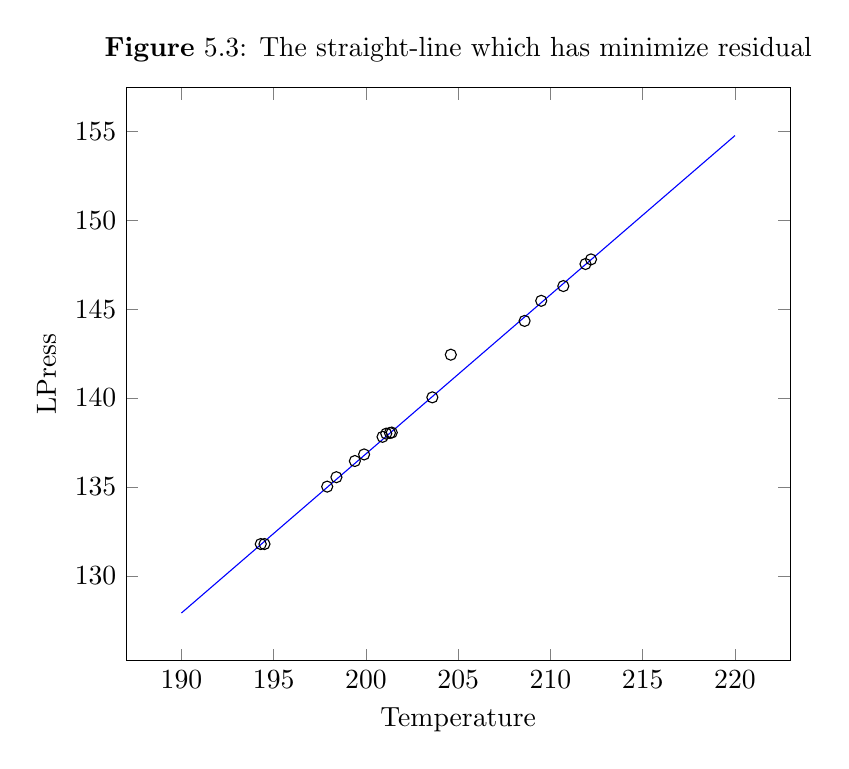
\begin{tikzpicture}
      \pgfplotsset{
          scale only axis,
      }
    
      \begin{axis}[
        title={\textbf{Figure} 5.3: The straight-line which has minimize residual},
        xlabel=Temperature,
        ylabel=LPress,
      ]
        \addplot[only marks, mark=o]
        coordinates{ % plot 1 data set
          (194.5,131.79)(194.3,131.79)(197.9,135.02)(198.4,135.55)(199.4,136.46)(199.9,136.83)(200.9,137.82)(201.1,138)(201.4,138.06)(201.3,138.04)(203.6,140.04)(204.6,142.44)(209.5,145.47)(208.6,144.34)(210.7,146.3)(211.9,147.54)(212.2,147.8)
          % more points...
        }; \label{plot_one}
        
        \addplot [color=blue, domain=190:220, mark=none] {-42.138+0.895*\x};
        
        % plot 1 legend entry
        \addlegendimage{/pgfplots/refstyle=plot_one}
      \end{axis}
    
    \end{tikzpicture}
    \end{center}

\section {Interpreting Regression Coefficients} 
    Firstly, we need to analysis the correlation between x and y by using the correlation analyze method with the main formula is the correlation coefficient. The result of the formula just evaluates whether or not there is a linear relationship, whether this relationship is positive or negative, stable or not.  
    
    The formula of the correlation coefficient is given from the Co-variance formula - which is also a method of evaluating the relationship between two variables x and y - but has a major limitation for which Co-variance formula is often rarely used and instead by the correlation coefficient. Specifically:
    
    \begin{align} 
        s_{xy} = \dfrac{\Sigma{(x_{i} - \overline{x})(y_{i} - \overline{y})}}{n - 1}\nonumber
    \end{align}
    
    For example, we have a sample data about the number of ad campaigns on Facebook per week for 10 weeks and how many million revenue cost (units of 1000 VND) are received, where x will be the number of campaigns per week, y is the sales


    \begin{center}
        \textbf{Table 6.1:} the number of ad campaigns on Facebook per week for 10 weeks
        
        \begin{tabular}{|c|c|c|}
            \hline 
            Week & Ad campaign & revenue cost  \\
            \hline
                1 & 2 & 4900 \\
                2 & 3 & 5100 \\ 
                3 & 5 & 5500 \\
                4 & 4 & 5100 \\
                5 & 1 & 3900 \\
                6 & 1 & 3600 \\
                7 & 3 & 4700 \\
                8 & 4 & 5500 \\
                9 & 2 & 4500 \\ 
                10 & 5 & 6000 \\
            \hline
        \end{tabular}
    \end{center}
    
    Next, we will apply the above-mentioned formula to calculate the co-variance is 1022. From there, we will divide the graph into 4 parts.
    
    \usepgfplotslibrary{fillbetween}
    \begin{center}
        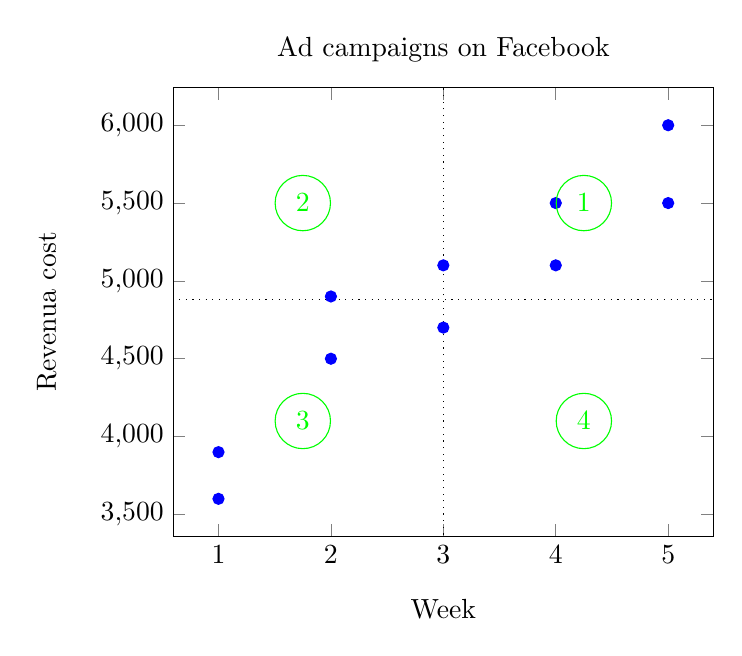
\begin{tikzpicture}
            \begin{axis}[
                title={Ad campaigns on Facebook},
                x label style={at={(axis description cs:0.5,-0.12)},anchor=north},
                y label style={at={(axis description cs:-0.2,0.5)},rotate=0,anchor=south},
                xlabel={Week},
                ylabel={Revenua cost},
            ]
            \draw [dotted] (3,0) -- (3,7000);
            \draw [dotted] (0,4880) -- (15,4880);
            \addplot[color=blue,only marks, mark=*]
            coordinates{
                (2,4900)(3,5100)(5, 5500)
                (4,5100)(1,3900)(1,3600)
                (3,4700)(4,5500)(2,4500)
                (5,6000)
            };
            \addplot[
            color=green,
            only marks,
            mark=o,
            mark size=10pt,
            nodes near coords={
                \pgfmathparse{int(\coordindex+1)}
                \pgfmathresult
            }, 
            every node near coord/.style={
                text=green,
                anchor=center
            }
            ]
            coordinates{
                (4.25,5500)[I]
                (1.75,5500)[II]
                (1.75,4100)[III]
                (4.25,4100)[IV]
            };
            \end{axis}  
        \end{tikzpicture}
    \end{center}
    
    Interpret the results: 
    
    The line in which value ${x = 4}$ is the average value over 10 weeks, the y line of ${10}$-week average revenue. This line divides the graph into four parts. Part 1 will have x value greater than average of ${x}$, ${y}$ greater than mean of y. Part 2 will have x value less than the mean of x and value of y greater than the mean of y. Similar to parts 3 and 4.
    
    Therefore, we can see (${x}$ - ${\overline{x}}$)(${y}$ - ${\overline{y}}$) will be positive with parts 1 and 3 but negative with parts 2 and 4. 
    
    \begin{itemize}
        \item If ${S_{xy}}$ is positive, the points are mostly in parts $1$ and $3$, a positive linear relationship. 
        \item If ${S_{xy}}$ is negative, the points are mostly in parts $2$ and $4$, a negative linear relationship. 
        \item If the points are completely divided equally into ${4}$ parts then ${S_{xy}}$ will be $0$ and there is no linear relationship between x and y. 
    \end{itemize}
    
    Looking on the graph we can see that 7/10 points are in parts 1 and 3 corresponding to positive S. From there, we can confirm that x and y have a linear relationship, which means that the advertising campaign increases, revenue also increases.

\section {Residual Checking} 

    \begin{multicols}{2}
    \begin{center}
    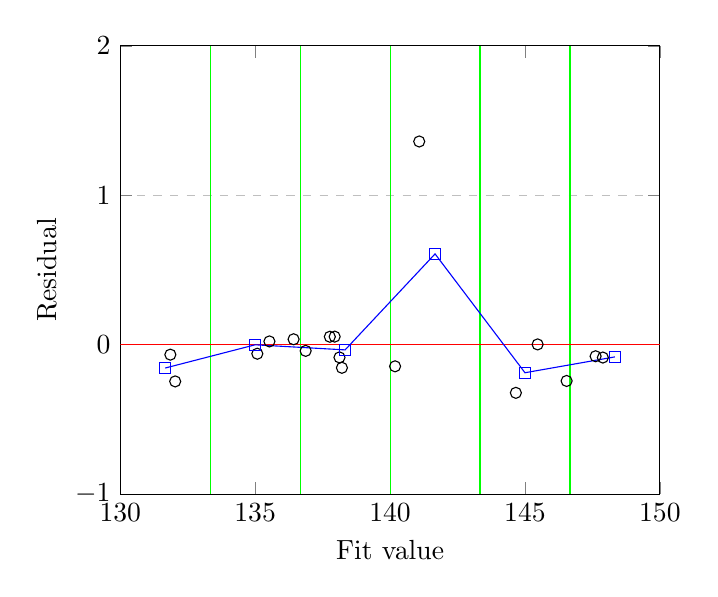
\begin{tikzpicture}
    \begin{axis}[
        title={},
        xlabel={Fit value},
        ylabel={Residual},
        xmin=130, xmax=150,
        ymin=-1, ymax=2,
        xtick={}, ytick={},
        legend pos=north west,
        ymajorgrids=true,
        grid style=dashed,
    ]
    
    \addplot[
        only marks, mark= o
        ]
        coordinates {
        (132.036,-0.245743)
        (131.857,-0.0666504)(135.08,-0.0604095)(135.528,0.0218506)
        (136.424,0.0363617)(136.871,-0.0413971)(137.767,0.0531158)
        (137.946,0.0540009)(138.215,-0.154633)(138.125,-0.0850983)
        (140.185,-0.144745)(141.08,1.35977)(145.468,0.00186157)
        (144.662,-0.322205)(146.543,-0.242722)(147.617,-0.0773315)
        (147.886,-0.085968)
        };
        \draw[color = green] (133.333,-1) -- (133.333,2) node[above] {$y$};
        \draw[color = green] (136.667,-1) -- (136.667,2) node[above] {$y$};
        \draw[color = green] (140,-1) -- (140,2) node[above] {$y$};
        \draw[color = green] (143.333,-1) -- (143.333,2) node[above] {$y$};
        \draw[color = green] (146.667,-1) -- (146.667,2) node[above] {$y$};
        \addplot [color=red, domain=130:150, mark=none] {0*\x};
        
        \addplot[
        color=blue,
        mark=square,
        ]
        coordinates {
        (131.667,-0.156197)
        (135,-0.000732422)
        (138.333,-0.0348022)
        (141.667,0.607513)
        (145,-0.187688)
        (148.333,-0.0816498)
        };
        
    \end{axis}
    \end{tikzpicture}
    \end{center} 
    
    \begin{center}
    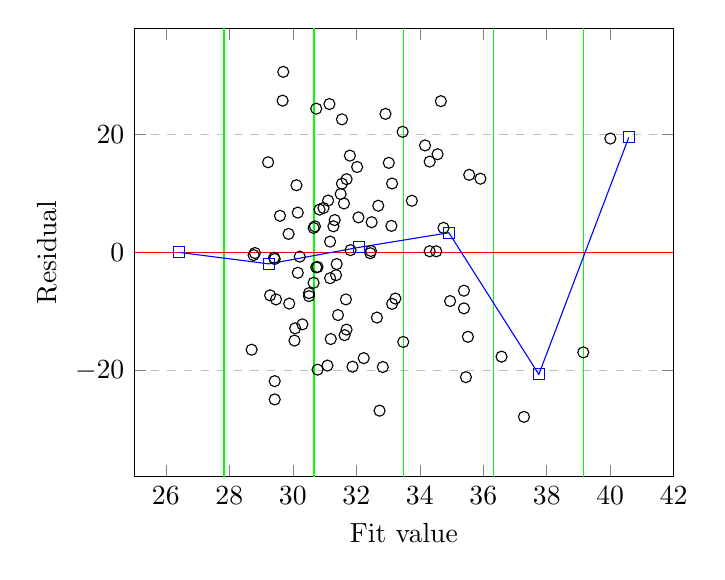
\begin{tikzpicture}
    \begin{axis}[
        title={},
        xlabel={Fit value},
        ylabel={Residual},
        xmin=25, xmax=42,
        ymin=-38, ymax=38,
        xtick={}, ytick={},
        legend pos=north west,
        ymajorgrids=true,
        grid style=dashed,
    ]
    
    \addplot[
        only marks, mark= o
        ]
        coordinates {
        (29.2219,15.2781)
        (31.8807,-19.3807)(31.3198,5.48015)(29.4296,-21.8296)
        (28.8064,-0.10644)(30.7798,-2.47978)(34.311,15.389)
        (30.0528,-14.9528)(34.5603,16.6397)(32.7323,-26.8323)
        (29.8658,3.13419)(31.5483,22.5517)(30.7382,-2.53823)
        (37.2814,-27.8814)(28.7649,-0.464897)(31.0914,-19.1914)
        (35.5573,13.1427)(31.1121,8.78787)(32.2338,-17.9338)
        (33.4594,20.4406)(31.4237,-10.6237)(31.673,-7.97297)
        (31.1537,25.1463)(31.5068,9.89321)(30.7798,-19.8798)
        (35.4535,-21.1535)(32.4623,0.237694)(31.1744,1.82556)
        (33.2309,-7.83087)(32.8362,-19.4362)(30.6967,4.40331)
        (30.5097,-6.90974)(31.1744,-4.37444)(29.2842,-7.28419)
        (28.7026,-16.5026)(31.1952,-14.6952)(31.7976,16.4024)
        (32.6493,-11.0493)(31.3614,-3.86139)(29.4088,-0.908827)
        (31.6937,-13.0937)(31.6937,12.4063)(32.4831,5.11692)
        (29.6789,25.7211)(29.6996,30.6004)(29.4296,-24.9296)
        (34.7472,4.15278)(34.5187,0.181271)(34.311,0.188992)
        (29.4711,-7.97114)(30.1566,-3.45662)(33.127,-8.72701)
        (31.2783,4.4217)(30.0735,-12.8735)(30.9667,7.53328)
        (32.0261,14.4739)(31.5483,11.6517)(29.4296,-1.1296)
        (33.127,11.673)(31.3822,-1.98216)(30.1151,11.3849)
        (32.0676,5.93236)(29.5958,6.20422)(30.6551,4.14486)
        (30.8421,7.25791)(29.8866,-8.68658)(30.6551,-5.15514)
        (34.9549,-8.25494)(30.5097,-7.40974)(32.6908,7.9092)
        (31.6107,8.28935)(35.5158,-14.3158)(35.3912,-9.49115)
        (36.5752,-17.6752)(30.1566,6.74338)(35.3912,-6.49115)
        (30.302,-12.202)(30.7382,24.3618)(34.1656,18.1344)
        (40.0025,19.2975)(30.2189,-0.718933)(31.6314,-14.0314)
        (33.0231,15.1769)(35.9104,12.4896)(31.8184,0.381626)
        (39.1509,-16.9509)(33.7502,8.74983)(34.6641,25.6359)
        (33.1062,4.49376)(32.9193,23.4807)(33.4801,-15.1801)
        (32.4415,-0.141533)
        };
        \draw[color = green] (27.8333,-38) -- (27.8333,38) node[above] {$y$};
        \draw[color = green] (30.6667,-38) -- (30.6667,38) node[above] {$y$};
        \draw[color = green] (33.5,-38) -- (33.5,38) node[above] {$y$};
        \draw[color = green] (36.3333,-38) -- (36.3333,38) node[above] {$y$};
        \draw[color = green] (39.1667,-38) -- (39.1667,38) node[above] {$y$};
    \addplot [color=red, domain=25:45, mark=none] {0*\x};
    
    \addplot[
        color=blue,
        mark=square,
        ]
        coordinates {
        (26.4167,0)
        (29.25,-1.94704)
        (32.0833,0.848493)
        (34.9167,3.33222)
        (37.75,-20.6881)
        (40.5833,19.4927)
        };
        
    \end{axis}
    \end{tikzpicture}
    \end{center}
    \end{multicols}
    
    \begin{multicols}{2}
    \begin{center}
    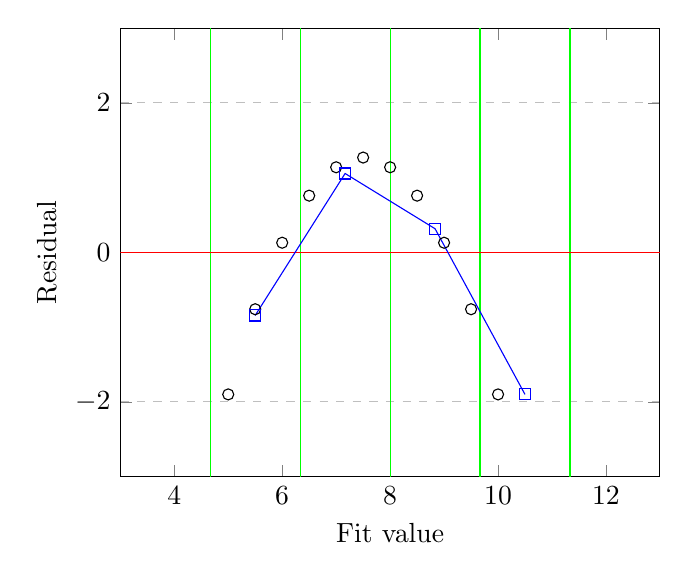
\begin{tikzpicture}
    \begin{axis}[
        title={},
        xlabel={Fit value},
        ylabel={Residual},
        xmin=3, xmax=13,
        ymin=-3, ymax=3,
        xtick={}, ytick={},
        legend pos=north west,
        ymajorgrids=true,
        grid style=dashed,
    ]
    
    \addplot[
        only marks, mark= o
        ]
        coordinates {
        (8.00091,1.13909)
        (7.00091,1.13909)(9.50091,-0.76091)(7.50091,1.26909)
        (8.50091,0.75909)(10.0009,-1.90091)(6.00091,0.129091)
        (5.00091,-1.90091)(9.00091,0.12909)(6.50091,0.759091)
        (5.50091,-0.76091)
        };
        \draw[color = green] (4.66667,-3) -- (4.66667,3) node[above] {$y$};
        \draw[color = green] (6.33333,-3) -- (6.33333,3) node[above] {$y$};
        \draw[color = green] (8,-3) -- (8,3) node[above] {$y$};
        \draw[color = green] (9.66667,-3) -- (9.66667,3) node[above] {$y$};
        \draw[color = green] (11.3333,-3) -- (11.3333,3) node[above] {$y$};
    \addplot [color=red, domain=3:13, mark=none] {0*\x};
    
    \addplot[
        color=blue,
        mark=square,
        ]
        coordinates {
        (5.5,-0.844243)
        (7.16667,1.05576)
        (8.83333,0.31659)
        (10.5,-1.90091)
        };
        
    \end{axis}
    \end{tikzpicture}
    \end{center}
    
    \begin{center}
    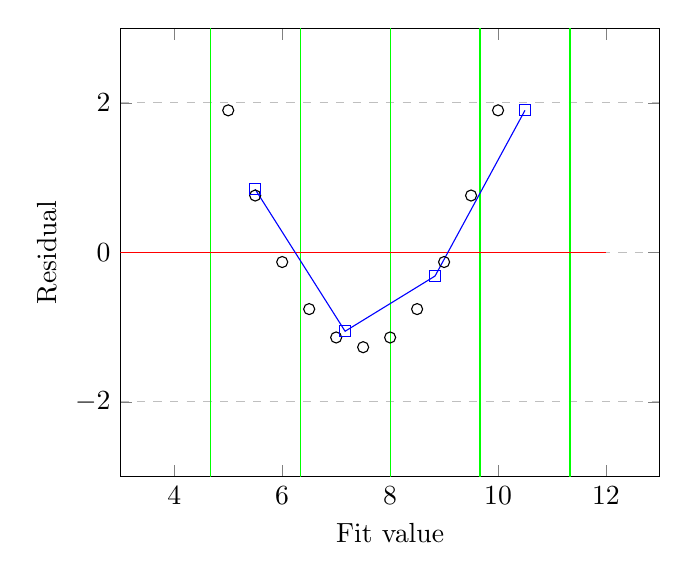
\begin{tikzpicture}
    \begin{axis}[
        title={},
        xlabel={Fit value},
        ylabel={Residual},
        xmin=3, xmax=13,
        ymin=-3, ymax=3,
        xtick={}, ytick={},
        legend pos=north west,
        ymajorgrids=true,
        grid style=dashed,
    ]
    
    \addplot[
        only marks, mark= o
        ]
        coordinates {
        (8.00091,-1.13909)
        (7.00091,-1.13909)(9.50091,0.76091)(7.50091,-1.26909)
        (8.50091,-0.75909)(10.0009,1.90091)(6.00091,-0.129091)
        (5.00091,1.90091)(9.00091,-0.12909)(6.50091,-0.759091)
        (5.50091,0.76091)
        };
        \draw[color = green] (4.66667,-3) -- (4.66667,3) node[above] {$y$};
        \draw[color = green] (6.33333,-3) -- (6.33333,3) node[above] {$y$};
        \draw[color = green] (8,-3) -- (8,3) node[above] {$y$};
        \draw[color = green] (9.66667,-3) -- (9.66667,3) node[above] {$y$};
        \draw[color = green] (11.3333,-3) -- (11.3333,3) node[above] {$y$};
    \addplot [color=red, domain=3:12, mark=none] {0*\x};
    
    \addplot[
        color=blue,
        mark=square,
        ]
        coordinates {
        (5.5,0.844243)
(7.16667,-1.05576)
(8.83333,-0.31659)
(10.5,1.90091)
        };
        
        
    \end{axis}
    \end{tikzpicture}
    \end{center}
    \end{multicols}
    
    \begin{center} 
         \textbf{Figure 7.1} Sample residual versus fit plots for testing equal variance
    \end{center}
    
    A plot of all residuals on the y-axis versus. the predicted values on the x-axis, called a residual versus fit plot, is a good way to check the linearity and equal variance assumptions. The fixed-x assumption can not be checked with residual analysis (or any other data analysis). 
    
     To analyze a residual vs. fit plot, such as any of the examples shown in \textbf{Figure 7.1}, you should mentally divide it up into about $5$ to $10$ vertical stripes (in here we will divide it into $5$ vertical stripes). Then each stripe represents all of the residuals for a number of subjects who have a similar predicted values.
     
     To check the linearity assumption, consider that for each $x$ value, if the mean of $Y$ falls on a straight line, then the residuals have a mean of \textbf{zero}. If we incorrectly fit a straight line to a curve, then some or most of the predicted means are incorrect, and this causes the residuals for at least specific ranges of $x$ (or the predicated $Y$ ) to be \textbf{non-zero} on average. Specifically if the data follow a simple curve, we will tend to have either a pattern of high then low then high residuals or the reverse. So the technique used to detect non-linearity in a residual vs. fit plot is to find the (vertical) mean of the residuals for each vertical stripe. 
     
     If the resultant connected segments or curve is close to a horizontal line at 0 on the y-axis, then we have no reason to doubt the linearity assumption. If there is a clear curve, most commonly a “smile” or “frown” shape, then we suspect non-linearity. 
     
     Four examples are shown in figure 7.1. In each band the mean residual is marked, and lines segments connect these. Plots A and B show no obvious pattern away from a horizontal line other that the small amount of expected “noise”. Plots C and D show clear deviations from normality, because the lines connecting the mean residuals of the vertical bands show a clear frown (C) and smile (D) pattern, rather than a flat line.
\end{document}

    
